\documentclass[12pt,a4paper]{report}

% =========================================================
% PACKAGES
% =========================================================
\usepackage[a4paper,margin=1in]{geometry}
\usepackage{setspace}
\usepackage{graphicx}
\usepackage{float}
\usepackage{booktabs}
\usepackage{array}
\usepackage{longtable}
\usepackage{xcolor}
\usepackage{listings}
\usepackage{hyperref}
\usepackage{fancyhdr}
\usepackage{titlesec}
\usepackage{enumitem}
\usepackage{caption}
\usepackage{amsmath}
\usepackage{amssymb}
\usepackage{tikz}
\usepackage{url}

\usetikzlibrary{positioning,arrows.meta,shapes.geometric}

% =========================================================
% DOCUMENT SETTINGS
% =========================================================

\onehalfspacing

\hypersetup{
    colorlinks=true,
    linkcolor=blue,
    urlcolor=blue,
    citecolor=blue
}

\pagestyle{fancy}
\fancyhf{}
\lhead{Software Maintenance Lab}
\rhead{Math Problem Solver}
\cfoot{\thepage}

\titleformat{\chapter}
{\normalfont\Huge\bfseries}
{\thechapter.}{1em}{}

\titleformat{\section}
{\normalfont\Large\bfseries}
{\thesection}{1em}{}

\titleformat{\subsection}
{\normalfont\large\bfseries}
{\thesubsection}{1em}{}

% =========================================================
% CODE STYLE
% =========================================================

\definecolor{codegray}{rgb}{0.95,0.95,0.95}
\definecolor{codegreen}{rgb}{0,0.45,0}
\definecolor{codeblue}{rgb}{0,0,0.65}

\lstset{
    backgroundcolor=\color{codegray},
    basicstyle=\ttfamily\small,
    keywordstyle=\color{codeblue}\bfseries,
    commentstyle=\color{codegreen},
    stringstyle=\color{red},
    breaklines=true,
    frame=single,
    numbers=left,
    numberstyle=\tiny,
    showstringspaces=false,
    tabsize=4
}

% =========================================================
% DOCUMENT
% =========================================================

\begin{document}

% =========================================================
% TITLE PAGE
% =========================================================

\begin{titlepage}
    \centering

    \vspace*{1cm}

    {\Large \textbf{ISLAMIC UNIVERSITY OF TECHNOLOGY}}\\[0.3cm]
    {\large \textbf{Department of Computer Science and Engineering}}\\[1.5cm]

    {\Huge \textbf{Software Maintenance Lab}}\\[0.5cm]


    {\Large \textbf{Project: Math Problem Solver}}\\[2cm]

    \begin{tabular}{ll}
        \textbf{Student Name:} & Muhammad Yasir Raiyan \\
        \textbf{Student ID:} & 210042152 \\
        \textbf{Course Title:} &  Software Maintenance Lab \\
        \textbf{Course Code:} &  SWE-4802 \\
        \textbf{Department:} & Computer Science and Engineering \\
        \textbf{Prog:} & B.S.C IN S.W.E \\
        \textbf{Semester:} & 8 \\
        \textbf{Academic Year:} & 2024-25\\
       
        
    \end{tabular}

    \vfill

    {\large \textbf{Academic Year: 2026}}

\end{titlepage}

% =========================================================
% TABLE OF CONTENTS
% =========================================================

\tableofcontents
\newpage

% =========================================================
% ABSTRACT
% =========================================================

\chapter*{Abstract}
\addcontentsline{toc}{chapter}{Abstract}

Software maintenance is an essential phase of the software
development life cycle because software systems must continuously
evolve after their initial development. Defects must be corrected,
software may need to operate in a new environment, internal quality
may need improvement, and users may require additional functionality.

This report presents the maintenance and analysis of a Python-based
application called \textit{Math Problem Solver}. The project was
developed as a Software Maintenance project and demonstrates four
major categories of software maintenance: corrective, adaptive,
preventive, and perfective maintenance.

Corrective maintenance was performed to address a division-by-zero
problem. Adaptive maintenance introduced a Flask-based web interface
to extend the command-line application to a web environment.
Preventive maintenance improved input validation, type information,
error handling, code organization, and maintainability. Perfective
maintenance extended the mathematical functionality of the system by
supporting operations such as factorial and percentage.

In addition, four transformation and software-analysis tools were
applied to the project: \textbf{Loguru}, \textbf{PySnooper},
\textbf{VizTracer}, and \textbf{SnakeViz}. These tools provide
different forms of information about the software. Loguru provides
application logging, PySnooper provides detailed execution tracing,
VizTracer provides runtime execution visualization, and SnakeViz
visualizes Python profiling information.

The final project was verified using Python's \texttt{unittest}
framework. The final test execution successfully passed 16 automated
tests. The project therefore demonstrates how maintenance activities,
testing, debugging, tracing, logging, and performance analysis can be
combined in a practical software maintenance workflow.

% =========================================================
% CHAPTER 1
% =========================================================

\chapter{Introduction}

\section{Background}

Software maintenance refers to the activities performed after the
initial development of a software system to keep the system
functional, reliable, maintainable, and useful.

A software system may require maintenance for several reasons.
Existing defects may need to be corrected, the execution environment
may change, the internal implementation may need improvement, or users
may request new functionality.

The project used in this laboratory is the
\textbf{Math Problem Solver}, a Python-based mathematical calculation
application. The project was progressively maintained and extended
through different maintenance activities.

The project also applies software analysis and transformation tools to
understand the behavior and performance of the maintained software.

\section{Project Objectives}

The main objectives of the project are:

\begin{itemize}
    \item To develop and maintain a mathematical calculation
    application.
    \item To demonstrate different categories of software maintenance.
    \item To identify and correct software defects.
    \item To adapt the application to a web-based environment.
    \item To improve code quality and maintainability.
    \item To add new mathematical features.
    \item To apply software analysis and transformation tools.
    \item To understand program execution and performance.
    \item To perform automated testing after maintenance activities.
\end{itemize}

\section{Assignment Objectives}

The laboratory assignment focuses on the following objectives:

\begin{itemize}
    \item Introduction to transformation and software analysis tools.
    \item Application of the tools to a working software project.
    \item Explanation of the insights obtained from tool outputs.
    \item Identification of maintenance scenarios where the tools can
    be used.
    \item Identification of alternative tools.
    \item Selection of preferred tools for future software projects.
\end{itemize}

% =========================================================
% CHAPTER 2
% =========================================================

\chapter{Project Overview}

\section{Math Problem Solver}

The Math Problem Solver is a Python-based mathematical calculation
application developed as a Software Maintenance project.

The original system was primarily command-line based. Through
successive maintenance activities, the project was improved and
extended.

The current project demonstrates:

\begin{itemize}
    \item Corrective Maintenance
    \item Adaptive Maintenance
    \item Preventive Maintenance
    \item Perfective Maintenance
    \item Program Comprehension
    \item Change Management
    \item Impact Analysis
    \item Reverse Engineering
    \item Refactoring
    \item Automated Testing
    \item Logging
    \item Execution Tracing
    \item Performance Profiling
\end{itemize}

\section{Technologies Used}

The project uses the following technologies and tools:

\begin{table}[H]
\centering
\caption{Technologies and Tools Used in the Project}
\begin{tabular}{p{4cm}p{8cm}}
\toprule
\textbf{Technology / Tool} & \textbf{Purpose} \\
\midrule
Python & Main programming language \\
Flask & Web-based adaptation \\
unittest & Automated testing \\
Loguru & Application logging \\
PySnooper & Debugging and execution tracing \\
VizTracer & Program execution tracing \\
cProfile & Python performance profiling \\
SnakeViz & Visualization of profiling results \\
Git & Version control \\
GitHub & Source-code repository \\
VS Code & Development environment \\
\bottomrule
\end{tabular}
\end{table}

These technologies are documented in the current project repository. :contentReference[oaicite:2]{index=2}

\section{Project Structure}

The current repository contains separate components for calculation,
testing, analysis, web presentation, utilities, and documentation.

The main project structure is:

\begin{lstlisting}
Math-Problem-Solver/
|
+-- Calculator/
|   +-- basic.py
|   +-- advanced.py
|   +-- validator.py
|
+-- Commands/
|
+-- Report/
|
+-- analysis/
|   +-- logging_demo.py
|   +-- pysnooper_demo.py
|   +-- viztrace_demo.py
|   +-- profile_demo.py
|
+-- templates/
|   +-- index.html
|
+-- tests/
|   +-- test_basic.py
|   +-- test_advaned.py
|   +-- test_integration.py
|   +-- test_validator.py
|
+-- utils/
|   +-- formatter.py
|   +-- logger.py
|
+-- app.py
+-- main.py
+-- Requirements.txt
+-- README.md
+-- LICENSE
\end{lstlisting}

The repository's current main branch lists the \texttt{Calculator},
\texttt{Commands}, \texttt{Report}, \texttt{analysis},
\texttt{templates}, \texttt{tests}, and \texttt{utils} directories,
along with the application and configuration files. :contentReference[oaicite:3]{index=3}

\section{Mathematical Functionality}

The final system supports the following mathematical operations:

\begin{enumerate}
    \item Addition
    \item Subtraction
    \item Multiplication
    \item Division
    \item Power
    \item Square Root
    \item Cube Root
    \item Factorial
    \item Percentage
\end{enumerate}

The repository documents these nine final mathematical operations. :contentReference[oaicite:4]{index=4}

% =========================================================
% CHAPTER 3
% =========================================================

\chapter{Software Maintenance Lifecycle}

\section{Maintenance Evolution}

The project follows the following maintenance sequence:

\[
V1
\rightarrow
V1.1
\rightarrow
V1.2
\rightarrow
V1.3
\rightarrow
V2.0
\]

The individual stages are:

\begin{enumerate}
    \item \textbf{V1}: Initial baseline system.
    \item \textbf{V1.1}: Corrective maintenance.
    \item \textbf{V1.2}: Adaptive maintenance.
    \item \textbf{V1.3}: Preventive maintenance.
    \item \textbf{V2.0}: Perfective maintenance and final system.
\end{enumerate}

\section{Maintenance Lifecycle Diagram}

\begin{figure}[H]
\centering
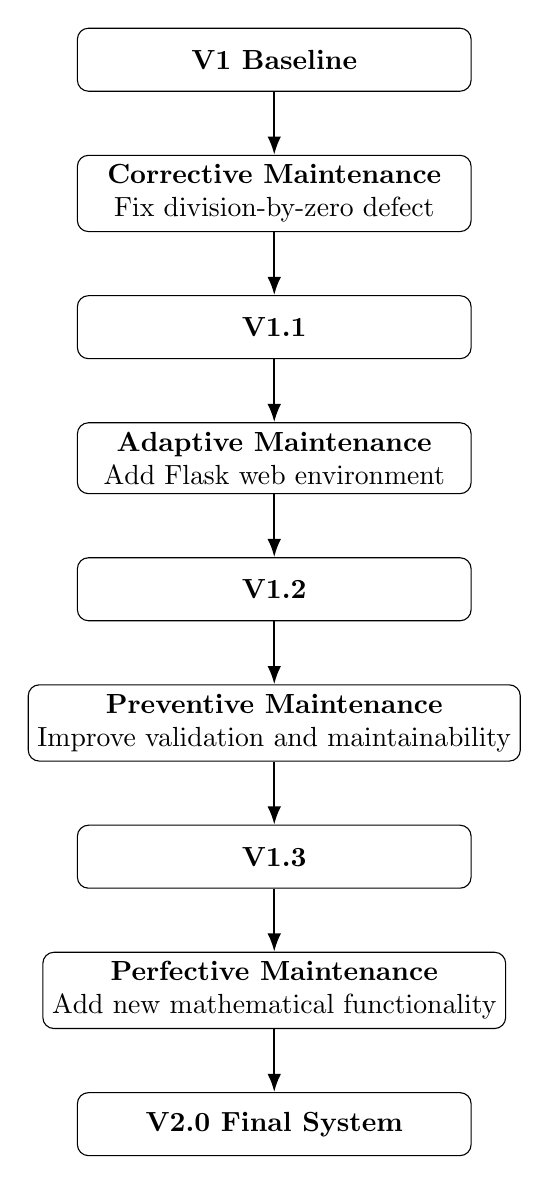
\begin{tikzpicture}[
    node distance=0.8cm,
    every node/.style={
        draw,
        rounded corners,
        align=center,
        minimum width=5.0cm,
        minimum height=0.8cm
    },
    arrow/.style={-{Latex}, thick}
]

\node (v1) {\textbf{V1 Baseline}};
\node (cm) [below=of v1] {\textbf{Corrective Maintenance}\\Fix division-by-zero defect};
\node (v11) [below=of cm] {\textbf{V1.1}};
\node (am) [below=of v11] {\textbf{Adaptive Maintenance}\\Add Flask web environment};
\node (v12) [below=of am] {\textbf{V1.2}};
\node (pm) [below=of v12] {\textbf{Preventive Maintenance}\\Improve validation and maintainability};
\node (v13) [below=of pm] {\textbf{V1.3}};
\node (pfm) [below=of v13] {\textbf{Perfective Maintenance}\\Add new mathematical functionality};
\node (v20) [below=of pfm] {\textbf{V2.0 Final System}};

\draw[arrow] (v1) -- (cm);
\draw[arrow] (cm) -- (v11);
\draw[arrow] (v11) -- (am);
\draw[arrow] (am) -- (v12);
\draw[arrow] (v12) -- (pm);
\draw[arrow] (pm) -- (v13);
\draw[arrow] (v13) -- (pfm);
\draw[arrow] (pfm) -- (v20);

\end{tikzpicture}
\caption{Software Maintenance Evolution}
\end{figure}

% =========================================================
% CHAPTER 4
% =========================================================

\chapter{Corrective Maintenance}

\section{Definition}

Corrective maintenance is performed to identify and fix defects or
errors found in existing software.

\section{Problem Identified}

A defect was identified in the division functionality.

When the denominator was zero, the application could produce a
\texttt{ZeroDivisionError}. This could terminate the operation
unexpectedly.

\section{Program Comprehension}

The original calculation flow was analyzed as follows:

\begin{lstlisting}
User
 |
 v
main.py
 |
 v
Calculator
 |
 v
divide(a,b)
 |
 v
a / b
\end{lstlisting}

The \texttt{divide()} function was identified as the location that
required correction.

\section{Change Management}

The requested change was:

\begin{quote}
Prevent division by zero and provide a meaningful error message.
\end{quote}

The function was modified to validate the denominator before
performing the division.

\begin{lstlisting}[language=Python]
def divide(a: float, b: float) -> float:
    if b == 0:
        raise ValueError("Cannot divide by zero")
    return a / b
\end{lstlisting}

\section{Impact Analysis}

The main affected components were:

\begin{itemize}
    \item Calculator division functionality -- direct impact.
    \item Main application -- indirect impact.
    \item Basic calculator test module -- regression testing.
\end{itemize}

\section{Reverse Engineering}

The original execution flow was reconstructed as:

\begin{lstlisting}
User
 |
 v
Select Division
 |
 v
main.py
 |
 v
divide(a,b)
 |
 v
Denominator = 0
 |
 v
ZeroDivisionError
\end{lstlisting}

After maintenance, the flow became:

\begin{lstlisting}
User
 |
 v
Select Division
 |
 v
divide(a,b)
 |
 v
Check denominator
 |
 +---- b == 0 ----> ValueError
 |
 +---- b != 0 ---> a / b
\end{lstlisting}

\section{Regression Test}

A regression test was added:

\begin{lstlisting}[language=Python]
def test_divide_by_zero(self):
    with self.assertRaises(ValueError):
        divide(10, 0)
\end{lstlisting}

\section{Testing Result}

Before corrective maintenance:

\[
10\text{ tests passed}
\]

After corrective maintenance:

\[
11\text{ tests passed}
\]

Therefore, the corrective maintenance was verified through automated
testing. The repository documents this transition from 10 to 11
successful tests. :contentReference[oaicite:5]{index=5}

\section{Version Evolution}

\[
V1
\rightarrow
\text{Corrective Maintenance}
\rightarrow
V1.1
\]

% =========================================================
% CHAPTER 5
% =========================================================

\chapter{Adaptive Maintenance}

\section{Definition}

Adaptive maintenance modifies software so that it can work in a
changed environment or support new environmental requirements.

\section{Problem}

The original application was primarily command-line based.

The system was required to support access through a web browser.

\section{Maintenance Action}

A Flask-based web interface was introduced while reusing the existing
calculator logic.

The adapted architecture became:

\begin{lstlisting}
Browser
 |
 v
index.html
 |
 v
app.py
 |
 v
Validation
 |
 v
Calculator Functions
 |
 v
Result
 |
 v
Browser
\end{lstlisting}

\section{Technology Added}

The adaptive maintenance introduced:

\begin{itemize}
    \item Flask
    \item HTML web interface
    \item Web application routing
\end{itemize}

\section{Impact Analysis}

The main affected components were:

\begin{itemize}
    \item \texttt{app.py} -- web application.
    \item \texttt{Requirements.txt} -- dependency configuration.
    \item \texttt{templates/index.html} -- web interface.
\end{itemize}

The existing calculator modules were reused rather than rewritten.

\section{Benefits}

The adaptive maintenance provides:

\begin{itemize}
    \item Browser-based access.
    \item Improved user interaction.
    \item Web-based execution.
    \item Better accessibility.
    \item Adaptation to a new execution environment.
\end{itemize}

\section{Version Evolution}

\[
V1.1
\rightarrow
\text{Adaptive Maintenance}
\rightarrow
V1.2
\]

The repository explicitly documents Flask as the web adaptation
technology and describes reuse of the existing calculator modules. :contentReference[oaicite:6]{index=6}

% =========================================================
% CHAPTER 6
% =========================================================

\chapter{Preventive Maintenance}

\section{Definition}

Preventive maintenance improves the internal quality of software to
reduce the possibility of future failures.

\section{Maintenance Activities}

The project was improved through:

\begin{itemize}
    \item Better input validation.
    \item Type hints.
    \item Improved error handling.
    \item Cleaner code organization.
    \item Improved maintainability.
\end{itemize}

For example, type hints make the expected input and output clearer:

\begin{lstlisting}[language=Python]
def add(a: float, b: float) -> float:
    return a + b
\end{lstlisting}

\section{Benefits}

The preventive maintenance activities help to:

\begin{itemize}
    \item Reduce future errors.
    \item Improve code readability.
    \item Improve maintainability.
    \item Make debugging easier.
    \item Improve software reliability.
\end{itemize}

\section{Version Evolution}

\[
V1.2
\rightarrow
\text{Preventive Maintenance}
\rightarrow
V1.3
\]

The current repository identifies input validation, type information,
error handling, and maintainability as the main preventive-maintenance
areas. :contentReference[oaicite:7]{index=7}

% =========================================================
% CHAPTER 7
% =========================================================

\chapter{Perfective Maintenance}

\section{Definition}

Perfective maintenance improves existing software by adding useful
features or improving functionality based on user requirements.

\section{Maintenance Action}

Additional mathematical functionality was introduced to make the
application more useful.

The final system supports:

\begin{itemize}
    \item Addition
    \item Subtraction
    \item Multiplication
    \item Division
    \item Power
    \item Square Root
    \item Cube Root
    \item Factorial
    \item Percentage
\end{itemize}

\section{Factorial}

Factorial can be represented mathematically as:

\[
n! = n(n-1)(n-2)\cdots 2(1)
\]

For example:

\[
5! = 5 \times 4 \times 3 \times 2 \times 1 = 120
\]

The factorial feature requires appropriate validation because
factorial is not defined for negative integers.

\section{Percentage}

The percentage operation can be represented as:

\[
\text{Percentage} =
\frac{\text{Value}\times\text{Percent}}{100}
\]

For example:

\[
20\% \text{ of } 500
=
\frac{500\times20}{100}
=
100
\]

\section{Benefits}

The additional functionality provides:

\begin{itemize}
    \item More mathematical operations.
    \item Greater usefulness to users.
    \item Improved application capability.
    \item A more complete mathematical calculator.
\end{itemize}

\section{Testing}

After adding the new functionality, the complete test suite was
executed.

The final result was:

\begin{lstlisting}
................
----------------------------------------------------------------------
Ran 16 tests in 0.002s

OK
\end{lstlisting}

\section{Version Evolution}

\[
V1.3
\rightarrow
\text{Perfective Maintenance}
\rightarrow
V2.0
\]

The current repository documents the final nine mathematical
operations and the 16-test result. :contentReference[oaicite:8]{index=8}

% =========================================================
% CHAPTER 8
% =========================================================

\chapter{Transformation and Analysis Tools}

\section{Overview}

The laboratory required the practical application of four tools:

\begin{enumerate}
    \item Loguru
    \item PySnooper
    \item VizTracer
    \item SnakeViz
\end{enumerate}

The tools provide different types of information.

\begin{table}[H]
\centering
\caption{Transformation and Analysis Tools}
\begin{tabular}{p{3cm}p{5cm}p{4cm}}
\toprule
\textbf{Tool} & \textbf{Primary Purpose} & \textbf{Main Output} \\
\midrule
Loguru & Logging and monitoring & Application events and errors \\
PySnooper & Debugging and tracing & Variables and execution flow \\
VizTracer & Runtime execution tracing & Visual execution timeline \\
SnakeViz & Profiling visualization & Performance information \\
\bottomrule
\end{tabular}
\end{table}

The four tools are explicitly documented in the current repository. :contentReference[oaicite:9]{index=9}

% =========================================================
% CHAPTER 9
% =========================================================

\chapter{Loguru}

\section{Introduction}

Loguru is a Python logging library that provides a simple way to
generate readable application logs.

In the Math Problem Solver project, Loguru is used to monitor
mathematical operations and application events.

\section{Usage in the Project}

A typical logging implementation can record the start and result of a
calculation:

\begin{lstlisting}[language=Python]
from loguru import logger

logger.add("logs/math_solver.log")

logger.info("Starting mathematical calculation")

result = add(4, 3)

logger.info("Addition result: {}", result)
\end{lstlisting}

The project analysis records an example similar to:

\begin{lstlisting}
[LOG] Addition operation performed
Addition result: 7.0
\end{lstlisting}

\section{Insight from Output}

The Loguru output provides a chronological record of application
activities.

From the example output, we can determine:

\begin{enumerate}
    \item The addition operation was executed.
    \item The operation completed successfully.
    \item The resulting value was 7.0.
\end{enumerate}

Therefore, Loguru answers the question:

\begin{quote}
\textbf{What happened during application execution?}
\end{quote}

\section{Maintenance Application}

Loguru is particularly useful during corrective maintenance.

Suppose a user reports that an operation is producing an unexpected
result. Logs can help the developer determine:

\begin{itemize}
    \item Which operation was executed.
    \item When the operation occurred.
    \item What result was produced.
    \item Whether an error occurred.
\end{itemize}

This reduces the need to reproduce every reported problem manually.

\section{Project Execution}

From the project root:

\begin{lstlisting}
python analysis\logging_demo.py
\end{lstlisting}

The repository documents this command for the Loguru demonstration. :contentReference[oaicite:10]{index=10}

% =========================================================
% CHAPTER 10
% =========================================================

\chapter{PySnooper}

\section{Introduction}

PySnooper is a Python debugging and execution-tracing tool.

It automatically records information about the execution of a
function, including variable values and return values.

\section{Usage in the Project}

A mathematical function can be traced using:

\begin{lstlisting}[language=Python]
import pysnooper

@pysnooper.snoop()
def calculate(a, b):
    result = a + b
    return result
\end{lstlisting}

A representative trace can contain:

\begin{lstlisting}
Starting var: a = 4
Starting var: b = 3
New var: result = 7
Return value: 7
\end{lstlisting}

\section{Insight from Output}

The output allows the developer to understand:

\begin{itemize}
    \item Which variables were created.
    \item The values stored in variables.
    \item How execution moved through the function.
    \item What value was returned.
\end{itemize}

Therefore, PySnooper answers:

\begin{quote}
\textbf{How did the function execute internally?}
\end{quote}

\section{Maintenance Application}

PySnooper is useful during corrective maintenance.

For example, if a percentage calculation returns an unexpected value,
the developer can trace the function and inspect its intermediate
variables.

This is especially helpful for understanding unfamiliar or legacy
code.

\section{Project Execution}

From the project root:

\begin{lstlisting}
python analysis\pysnooper_demo.py
\end{lstlisting}

The repository specifies this command for the PySnooper analysis. :contentReference[oaicite:11]{index=11}

% =========================================================
% CHAPTER 11
% =========================================================

\chapter{VizTracer}

\section{Introduction}

VizTracer is a Python execution-tracing tool that records program
execution and allows developers to visualize the execution flow.

It is useful when the developer needs more than textual logging.

\section{Usage in the Project}

The project contains a VizTracer demonstration script.

The command used is:

\begin{lstlisting}
viztracer analysis\viztrace_demo.py
\end{lstlisting}

VizTracer generates trace information that can be inspected using its
visualization interface.

\section{Information Provided}

The visualization can show:

\begin{itemize}
    \item Function calls.
    \item Execution sequence.
    \item Execution duration.
    \item Repeated operations.
    \item Program execution flow.
\end{itemize}

A simplified execution relationship can be represented as:

\begin{lstlisting}
main()
 |
 +---- add()
 |
 +---- logger
 |
 +---- result
\end{lstlisting}

\section{Insight from Output}

VizTracer provides a dynamic view of program behavior.

It helps answer:

\begin{quote}
\textbf{When and in what order did different parts of the program execute?}
\end{quote}

This is useful for understanding interactions between application
components.

\section{Maintenance Application}

VizTracer can support corrective and preventive maintenance.

For example, suppose a future version of the web application becomes
slower. The execution trace can help identify:

\begin{itemize}
    \item Repeated function calls.
    \item Long-running functions.
    \item Unexpected execution paths.
    \item Functions requiring optimization.
\end{itemize}

\section{Project Execution}

If necessary, VizTracer can be installed using:

\begin{lstlisting}
pip install viztracer
\end{lstlisting}

Then the demonstration can be executed using:

\begin{lstlisting}
viztracer analysis\viztrace_demo.py
\end{lstlisting}

These commands are documented in the current repository. :contentReference[oaicite:12]{index=12}

% =========================================================
% CHAPTER 12
% =========================================================

\chapter{SnakeViz}

\section{Introduction}

SnakeViz is a visualization tool for Python profiling information
generated by \texttt{cProfile}.

Unlike ordinary logging, profiling focuses on execution statistics and
performance.

\section{Profiling Process}

The project first generates profiling data:

\begin{lstlisting}
python -m cProfile -o profile.prof analysis\profile_demo.py
\end{lstlisting}

The resulting profile can then be visualized with:

\begin{lstlisting}
snakeviz profile.prof
\end{lstlisting}

\section{Insight from Output}

SnakeViz provides visual information about:

\begin{itemize}
    \item Number of function calls.
    \item Total execution time.
    \item Cumulative execution time.
    \item Functions consuming significant execution time.
    \item Potential performance bottlenecks.
\end{itemize}

Therefore, SnakeViz answers:

\begin{quote}
\textbf{Where is execution time being spent?}
\end{quote}

\section{Maintenance Application}

SnakeViz is particularly useful for preventive and perfective
maintenance.

For example, after adding new mathematical features, profiling can be
used to determine whether any function has introduced unnecessary
execution overhead.

A developer can then focus optimization efforts on the functions that
require improvement.

\section{Project Execution}

If necessary, SnakeViz can be installed using:

\begin{lstlisting}
pip install snakeviz
\end{lstlisting}

Then:

\begin{lstlisting}
python -m cProfile -o profile.prof analysis\profile_demo.py
snakeviz profile.prof
\end{lstlisting}

The current repository documents this profiling workflow. :contentReference[oaicite:13]{index=13}

% =========================================================
% CHAPTER 13
% =========================================================

\chapter{Analysis of Tool Outputs}

\section{Different Types of Insights}

The four tools provide complementary information.

\begin{table}[H]
\centering
\caption{Output Insights}
\begin{tabular}{p{3cm}p{8cm}}
\toprule
\textbf{Tool} & \textbf{Insight} \\
\midrule
Loguru & What application event happened and what result/error was recorded. \\
PySnooper & How a function executed and how its variables changed. \\
VizTracer & When functions executed, in what order, and for how long. \\
SnakeViz & Which functions consumed execution time and where potential bottlenecks exist. \\
\bottomrule
\end{tabular}
\end{table}

\section{Conceptual Relationship}

The tools can be summarized as:

\[
\boxed{\text{Loguru} \rightarrow \text{What happened?}}
\]

\[
\boxed{\text{PySnooper} \rightarrow \text{How did it happen?}}
\]

\[
\boxed{\text{VizTracer} \rightarrow \text{When and in what order?}}
\]

\[
\boxed{\text{SnakeViz} \rightarrow \text{Where is time spent?}}
\]

Together, these tools provide a broader understanding of the existing
system.

\section{Maintenance Mapping}

\begin{table}[H]
\centering
\caption{Tool and Maintenance Mapping}
\begin{tabular}{p{4cm}p{3cm}p{5cm}}
\toprule
\textbf{Maintenance Type} & \textbf{Tool} & \textbf{Example Usage} \\
\midrule
Corrective & Loguru & Find application errors and events \\
Corrective & PySnooper & Trace incorrect calculations \\
Corrective & VizTracer & Inspect unexpected execution paths \\
Preventive & PySnooper & Understand code before refactoring \\
Preventive & VizTracer & Analyze execution behavior \\
Preventive & SnakeViz & Identify possible performance bottlenecks \\
Perfective & SnakeViz & Analyze newly added functionality \\
Adaptive & Loguru & Monitor new web functionality \\
\bottomrule
\end{tabular}
\end{table}

The repository similarly maps Loguru, PySnooper, VizTracer, and SnakeViz
to different maintenance activities. :contentReference[oaicite:14]{index=14}

% =========================================================
% CHAPTER 14
% =========================================================

\chapter{Transformation Tool Simulation}

\section{Simulation in the Math Problem Solver}

The tools were not considered only as theoretical concepts. They were
applied to the Math Problem Solver project through dedicated analysis
scripts.

The simulation can be represented as:

\begin{lstlisting}
                    Math Problem Solver
                            |
          +-----------------+-----------------+
          |                 |                 |
        Loguru           PySnooper        VizTracer
          |                 |                 |
     Application       Execution         Execution
       Logging          Tracing         Visualization
                            |
                         SnakeViz
                            |
                    Performance Profiling
\end{lstlisting}

\section{Loguru Simulation}

The Loguru demonstration executes mathematical operations and records
application events.

Example:

\begin{lstlisting}
python analysis\logging_demo.py
\end{lstlisting}

Expected type of output:

\begin{lstlisting}
[LOG] Addition operation performed
Addition result: 7.0
\end{lstlisting}

\section{PySnooper Simulation}

The PySnooper demonstration traces function execution.

\begin{lstlisting}
python analysis\pysnooper_demo.py
\end{lstlisting}

Expected information includes:

\begin{lstlisting}
Starting var: a = 4
Starting var: b = 3
New var: result = 7
Return value: 7
\end{lstlisting}

\section{VizTracer Simulation}

The VizTracer demonstration records execution information:

\begin{lstlisting}
viztracer analysis\viztrace_demo.py
\end{lstlisting}

The generated visualization allows inspection of:

\begin{itemize}
    \item Function execution order.
    \item Function duration.
    \item Execution timeline.
    \item Repeated calls.
\end{itemize}

\section{SnakeViz Simulation}

Profiling information is generated using:

\begin{lstlisting}
python -m cProfile -o profile.prof analysis\profile_demo.py
\end{lstlisting}

The result is visualized using:

\begin{lstlisting}
snakeviz profile.prof
\end{lstlisting}

The visualization provides function call counts, execution time,
cumulative time, and potential performance bottlenecks.

\section{Complete Simulation Sequence}

The complete sequence from the project root is:

\begin{lstlisting}
python main.py

python -m unittest discover -s tests -p "test_*.py"

python analysis\logging_demo.py

python analysis\pysnooper_demo.py

viztracer analysis\viztrace_demo.py

python -m cProfile -o profile.prof analysis\profile_demo.py

snakeviz profile.prof
\end{lstlisting}

The current repository documents this complete analysis command
sequence. :contentReference[oaicite:15]{index=15}

% =========================================================
% CHAPTER 15
% =========================================================

\chapter{Alternatives to the Selected Tools}

\section{Alternatives to Loguru}

Possible alternatives include:

\begin{itemize}
    \item Python built-in \texttt{logging}
    \item Structlog
    \item Logbook
\end{itemize}

The built-in Python \texttt{logging} module is a strong alternative
because it is part of the Python standard library and does not require
an additional external package.

\section{Alternatives to PySnooper}

Possible alternatives include:

\begin{itemize}
    \item \texttt{pdb}
    \item VS Code Debugger
    \item Python \texttt{breakpoint()}
\end{itemize}

The VS Code Debugger is especially useful for interactive debugging
because it supports breakpoints, variable inspection, call-stack
inspection, and step-by-step execution.

\section{Alternatives to VizTracer}

Possible alternatives include:

\begin{itemize}
    \item Pyinstrument
    \item cProfile
    \item Yappi
\end{itemize}

These tools can provide different forms of execution and performance
analysis.

\section{Alternatives to SnakeViz}

Possible alternatives include:

\begin{itemize}
    \item Pyinstrument
    \item Py-Spy
    \item Tuna
\end{itemize}

These tools provide alternative approaches to Python profiling and
performance visualization.

The alternatives listed above are consistent with the alternatives
documented in the project's current README. :contentReference[oaicite:16]{index=16}

% =========================================================
% CHAPTER 16
% =========================================================

\chapter{Preferred Tools for Future Projects}

\section{Preferred Logging Tool: Loguru}

For a small-to-medium Python application, I would prefer Loguru for
application logging because of its simple syntax and readable output.

For larger systems with strict infrastructure requirements, Python's
built-in logging framework may be preferable because of its standard
library integration and extensive configuration options.

For the Math Problem Solver project, Loguru is convenient and easy to
use.

\section{Preferred Debugging Tool: VS Code Debugger}

For interactive debugging, I would prefer the VS Code Debugger.

Important features include:

\begin{itemize}
    \item Breakpoints.
    \item Variable inspection.
    \item Step-by-step execution.
    \item Call-stack inspection.
    \item Interactive debugging.
\end{itemize}

PySnooper is still valuable when a lightweight textual execution trace
is preferred.

\section{Preferred Runtime Analysis Tool: VizTracer}

VizTracer is useful when a developer wants a visual representation of
program execution.

It is particularly useful for understanding:

\begin{itemize}
    \item Function relationships.
    \item Execution order.
    \item Runtime duration.
    \item Repeated operations.
\end{itemize}

\section{Preferred Profiling Tool: SnakeViz}

For projects using Python's \texttt{cProfile}, SnakeViz is a convenient
tool for visualizing the resulting profiling data.

It makes profiling information easier to interpret than raw textual
statistics.

\section{Overall Preference}

For a future Python software project, my preferred combination would
be:

\begin{table}[H]
\centering
\caption{Preferred Toolset}
\begin{tabular}{p{4cm}p{7cm}}
\toprule
\textbf{Purpose} & \textbf{Preferred Tool} \\
\midrule
Application Logging & Loguru \\
Interactive Debugging & VS Code Debugger \\
Runtime Execution Analysis & VizTracer \\
Profiling Visualization & SnakeViz \\
Automated Testing & unittest / pytest \\
\bottomrule
\end{tabular}
\end{table}

The repository also identifies Loguru, VS Code Debugger, VizTracer,
and SnakeViz as preferred tools for different future-project
requirements. :contentReference[oaicite:17]{index=17}

% =========================================================
% CHAPTER 17
% =========================================================

\chapter{Testing and Verification}

\section{Testing Framework}

The project uses Python's \texttt{unittest} framework for automated
testing.

The test suite covers the maintained mathematical functionality and
integration behavior.

\section{Test Command}

The complete test suite is executed using:

\begin{lstlisting}
python -m unittest discover -s tests -p "test_*.py"
\end{lstlisting}

\section{Final Test Result}

The final result was:

\begin{lstlisting}
................
----------------------------------------------------------------------
Ran 16 tests in 0.002s

OK
\end{lstlisting}

Therefore:

\[
\boxed{16\text{ tests passed successfully}}
\]

The repository records the final result as 16 successful automated
tests. :contentReference[oaicite:18]{index=18}

\section{Importance of Regression Testing}

Regression testing is important after software maintenance because a
change in one part of the application may unintentionally affect
another part.

For example:

\begin{itemize}
    \item Corrective maintenance required testing division behavior.
    \item Adaptive maintenance required ensuring that calculator
    functionality remained reusable.
    \item Preventive maintenance required checking validation and
    existing functionality.
    \item Perfective maintenance required testing newly added
    operations.
\end{itemize}

The successful final test suite provides evidence that the tested
functionality remained operational after the maintenance changes.

% =========================================================
% CHAPTER 18
% =========================================================

\chapter{Running the Project}

\section{Clone the Repository}

The project repository is hosted on GitHub.

\begin{lstlisting}
git clone https://github.com/Yasirraiyan/
210042152-SWE-4802-Software-Maintainance-Lab-Project.git
\end{lstlisting}

Then:

\begin{lstlisting}
cd 210042152-SWE-4802-Software-Maintainance-Lab-Project
\end{lstlisting}

\section{Create Virtual Environment}

On Windows PowerShell:

\begin{lstlisting}
python -m venv venv
\end{lstlisting}

Activate the virtual environment:

\begin{lstlisting}
.\venv\Scripts\Activate.ps1
\end{lstlisting}

After successful activation, the terminal displays:

\begin{lstlisting}
(venv)
\end{lstlisting}

\section{Install Dependencies}

The repository uses a \texttt{Requirements.txt} file.

From the project root:

\begin{lstlisting}
python -m pip install -r Requirements.txt
\end{lstlisting}

\section{Run Main Application}

The main command-line application can be executed using:

\begin{lstlisting}
python main.py
\end{lstlisting}

A typical interaction is:

\begin{lstlisting}
===== Math Problem Solver =====
1. Addition
2. Subtraction
3. Multiplication
4. Division
5. Square Root
6. Cube Root
7. Power

Enter your choice: 1
Enter first number: 4
Enter second number: 3

Addition result: 7.0
\end{lstlisting}

The current repository documents the main application command and
example output. :contentReference[oaicite:19]{index=19}

\section{Run Tests}

Use:

\begin{lstlisting}
python -m unittest discover -s tests -p "test_*.py"
\end{lstlisting}

Expected final result:

\begin{lstlisting}
................
----------------------------------------------------------------------
Ran 16 tests in 0.002s

OK
\end{lstlisting}

% =========================================================
% CHAPTER 19
% =========================================================

\chapter{Importance of Analysis Tools in Maintenance}

Software maintenance becomes easier when developers understand how an
existing system behaves.

The selected tools provide different forms of evidence.

\section{Loguru}

Loguru provides evidence about application events.

\[
\text{Loguru} \Rightarrow \text{What happened?}
\]

\section{PySnooper}

PySnooper provides evidence about detailed function execution.

\[
\text{PySnooper} \Rightarrow \text{How did the code execute?}
\]

\section{VizTracer}

VizTracer provides evidence about execution sequence and timing.

\[
\text{VizTracer} \Rightarrow
\text{When and in what order did execution occur?}
\]

\section{SnakeViz}

SnakeViz provides evidence about profiling and execution cost.

\[
\text{SnakeViz} \Rightarrow
\text{Where is execution time being spent?}
\]

\section{Maintenance Benefits}

Together, the tools help developers:

\begin{itemize}
    \item Debug existing defects.
    \item Understand unfamiliar code.
    \item Monitor application behavior.
    \item Trace execution paths.
    \item Find potential performance bottlenecks.
    \item Support refactoring.
    \item Improve maintainability.
    \item Validate changes.
    \item Support future software evolution.
\end{itemize}

% =========================================================
% CHAPTER 20
% =========================================================

\chapter{Overall Project Status}

The project evolved from a basic command-line mathematical
application into a more complete and maintainable software system.

\begin{table}[H]
\centering
\caption{Final Project Evolution}
\begin{tabular}{p{3cm}p{7cm}}
\toprule
\textbf{Version} & \textbf{Major Change} \\
\midrule
V1 & Initial baseline mathematical application \\
V1.1 & Corrective maintenance -- division-by-zero handling \\
V1.2 & Adaptive maintenance -- Flask web interface \\
V1.3 & Preventive maintenance -- validation and maintainability improvements \\
V2.0 & Perfective maintenance -- additional mathematical features \\
\bottomrule
\end{tabular}
\end{table}

\section{Final Features}

The final project provides:

\begin{itemize}
    \item Addition.
    \item Subtraction.
    \item Multiplication.
    \item Division.
    \item Power.
    \item Square root.
    \item Cube root.
    \item Factorial.
    \item Percentage.
    \item Input validation.
    \item Error handling.
    \item Logging.
    \item Automated testing.
    \item Web adaptation.
    \item Execution analysis.
    \item Performance profiling.
\end{itemize}

The current repository identifies these features and analysis
capabilities as part of the final project. :contentReference[oaicite:20]{index=20}

% =========================================================
% CHAPTER 21
% =========================================================

\chapter{Discussion}

The Math Problem Solver provides a practical example of how a
relatively small software system can undergo multiple maintenance
activities.

Corrective maintenance addressed an existing defect. Adaptive
maintenance changed the environment in which the application could be
used. Preventive maintenance improved internal software quality, and
perfective maintenance added new user-oriented functionality.

The transformation and analysis tools complement these maintenance
activities.

Loguru is useful for monitoring application events. PySnooper is
useful for understanding detailed execution inside functions.
VizTracer provides a visual representation of runtime behavior.
SnakeViz provides an intuitive view of profiling information.

Using several tools is useful because each tool provides a different
perspective.

For example:

\[
\text{Loguru}
+
\text{PySnooper}
+
\text{VizTracer}
+
\text{SnakeViz}
\]

provides a combination of:

\begin{itemize}
    \item Application-level information.
    \item Function-level information.
    \item Runtime execution information.
    \item Performance information.
\end{itemize}

This combination supports software developers throughout the
maintenance lifecycle.

% =========================================================
% CHAPTER 22
% =========================================================

\chapter{Conclusion}

This report presented the maintenance and analysis of the Math Problem
Solver project.

The project demonstrated four major software maintenance categories.

First, corrective maintenance was used to fix the division-by-zero
defect. Second, adaptive maintenance introduced a Flask-based web
interface so that the application could operate in a web environment.
Third, preventive maintenance improved validation, type information,
error handling, code organization, and maintainability. Finally,
perfective maintenance expanded the functionality of the application
with additional mathematical operations.

The report also demonstrated four transformation and software analysis
tools: Loguru, PySnooper, VizTracer, and SnakeViz.

Loguru provides application logging and helps identify what happened
during execution. PySnooper provides detailed function-level tracing
and helps explain how execution occurred. VizTracer provides a runtime
execution timeline and helps developers understand program behavior.
SnakeViz visualizes profiling information and helps identify possible
performance bottlenecks.

The tools were applied to the Math Problem Solver rather than being
considered only theoretically. Dedicated analysis scripts were used
for logging, tracing, execution visualization, and profiling.

Finally, the project was verified through automated testing. The final
test suite successfully passed 16 tests.

Therefore, the project successfully demonstrates how software can be
maintained, analyzed, debugged, tested, improved, and extended
throughout its lifecycle.

% =========================================================
% REFERENCES
% =========================================================

\begin{thebibliography}{9}

\bibitem{github}
Yasir Raiyan,
\textit{210042152-SWE-4802-Software-Maintainance-Lab-Project},
GitHub Repository, 2026.

\url{https://github.com/Yasirraiyan/210042152-SWE-4802-Software-Maintainance-Lab-Project}

\bibitem{loguru}
Loguru Documentation,
\textit{Python Logging Made (Stupidly) Simple}.

\url{https://loguru.readthedocs.io/}

\bibitem{pysnooper}
PySnooper,
\textit{Python Debugging and Execution Tracing Tool}.

\url{https://github.com/cool-RR/PySnooper}

\bibitem{viztracer}
VizTracer Documentation,
\textit{A Debugging and Profiling Tool for Python}.

\url{https://viztracer.readthedocs.io/}

\bibitem{snakeviz}
SnakeViz Documentation,
\textit{Web-based Viewer for Python Profiler Output}.

\url{https://jiffyclub.github.io/snakeviz/}

\bibitem{python}
Python Documentation,
\textit{The Python Standard Library}.

\url{https://docs.python.org/3/library/}

\end{thebibliography}

% =========================================================
% APPENDIX
% =========================================================

\appendix

\chapter{Complete Command Reference}

\section{Environment Setup}

\begin{lstlisting}
python -m venv venv
.\venv\Scripts\Activate.ps1
python -m pip install -r Requirements.txt
\end{lstlisting}

\section{Run Application}

\begin{lstlisting}
python main.py
\end{lstlisting}

\section{Run Tests}

\begin{lstlisting}
python -m unittest discover -s tests -p "test_*.py"
\end{lstlisting}

\section{Run Loguru}

\begin{lstlisting}
python analysis\logging_demo.py
\end{lstlisting}

\section{Run PySnooper}

\begin{lstlisting}
python analysis\pysnooper_demo.py
\end{lstlisting}

\section{Run VizTracer}

\begin{lstlisting}
pip install viztracer
viztracer analysis\viztrace_demo.py
\end{lstlisting}

\section{Run SnakeViz}

\begin{lstlisting}
pip install snakeviz
python -m cProfile -o profile.prof analysis\profile_demo.py
snakeviz profile.prof
\end{lstlisting}

\section{Final Test Evidence}

\begin{lstlisting}
................
----------------------------------------------------------------------
Ran 16 tests in 0.002s

OK
\end{lstlisting}

\end{document}
